\documentclass[11pt,a4paper]{article}

\def\nyear {2025}
\def\nterm {Spring}
\def\nlecturer {}
\def\ncourse {Miscellaneous Projects}

\makeatletter

% packages
\usepackage{amssymb,amsfonts,amsmath,calc,tikz,pgfplots,geometry,mathtools}
\usepackage{color}   % May be necessary if you want to color links
\usepackage[svgnames]{xcolor}
\usepackage[hidelinks]{hyperref}
\usepackage{forest}
\usepackage{commath} % ew
\usepackage{esvect} % \vv makes vectors
\usepackage{centernot} % for the comparison
\usepackage{esdiff}
\usepackage{esint}
\usepackage{amsthm}
\usepackage{fancyhdr}
\usepackage{bm}
\usepackage{witharrows}
\usepackage{bookmark}
\usepackage{tikz-cd}
\usepackage{quiver}
\usepackage{bbm}
\usepackage{textcomp}
\usepackage{float}
\usepackage{gensymb}
\usepackage{cleveref}
\usepackage{environ}
\usepackage{comment}
\usepackage{cancel}
\usepackage{xparse}

% Inevitable cs
\usepackage{listings}
\usepackage[]{algorithm2e}

% tikz libraries
\usetikzlibrary{positioning}
\usetikzlibrary{matrix}
\usetikzlibrary{arrows}
\usetikzlibrary{bending}
\usetikzlibrary{arrows.meta}
\usetikzlibrary{decorations.markings}
\usetikzlibrary{decorations.pathreplacing}
\usetikzlibrary{decorations.markings}
\usetikzlibrary{patterns}
\usetikzlibrary{backgrounds}

% Page style setup
\pagestyle{fancy}
\fancyhfoffset{0pt}
\renewcommand{\headwidth}{\textwidth}
\geometry{margin=1in}
\pgfplotsset{compat=1.18}
\setlength{\headheight}{14.6pt}
\addtolength{\topmargin}{-1.6pt}
\hypersetup{
    colorlinks=false,
    linktoc=section,
    linkcolor=black,
}

%% maketitle setup
\ifx \nauthor\undefined
  \def\nauthor{Yeheli Fomberg}
\else
\fi

\ifx \nemail\undefined
  \def\nemail{\href{mailto:yp@campus.technion.ac.il}
  {\texttt{<yp@campus.technion.ac.il>}}}
\else
\fi

\ifx \ncoursehead \undefined
  \def\ncoursehead{\ncourse}
\fi

\lhead{\emph{\nouppercase{\leftmark}}}
\ifx \nextra \undefined
  \rhead{
    \ifnum\thepage=1
    \else
      \ncoursehead
    \fi}
\else
  \rhead{
    \ifnum\thepage=1
    \else
      \ncoursehead \ (\nextra)
    \fi}
\fi

\def\notes{notes}
\def\problems{problems}

\ifx \ntype \undefined
  \def\ntype{notes}
\else
\fi

\ifx \ntype \notes
  \let\@real@maketitle\maketitle
  \renewcommand{\maketitle}{\@real@maketitle\begin{center}
  \begin{minipage}[c]{0.9\textwidth}\centering\footnotesize
  These notes are not endorsed by the lecturers.
  I have revised them outside lectures to incorporate supplementary
  explanations, clarifications, and material for fun.
  While I have strived for accuracy, any errors or misinterpretations 
  are most likely mine.
  \end{minipage}\end{center}}
\else
  \ifx \ntype \problems
    \let\@real@maketitle\maketitle
    \renewcommand{\maketitle}{\@real@maketitle\begin{center}
    \begin{minipage}[c]{0.9\textwidth}\centering\footnotesize
    These problems are mostly based on the problem sets I was given
    when taking the course.
    
    While I have strived for accuracy and completeness,
    some of the problems would not have been here without the help of
    friends.
    \end{minipage}\end{center}}
  \else
  \fi
\fi


% theorem environments
\theoremstyle{definition}
\newtheorem{definition}{Definition}[section]
\newtheorem{remark}{Remark}[section]
\newtheorem{example}{Example}[section]
\newtheorem{exercise}{Exercise}[section]
\newtheorem{paradox}{Paradox}[section]
\newtheorem{entry}{Entry}[section]
\newtheorem*{solution}{Solution}
\newtheorem*{question}{Question}
\newtheorem*{answer}{Answer}
\newtheorem*{problem}{Problem}
\theoremstyle{plain}
\newtheorem{theorem}{Theorem}[section]
\newtheorem{proposition}[theorem]{Proposition}
\newtheorem{lemma}[theorem]{Lemma}
\newtheorem{corollary}[theorem]{Corollary}
\newenvironment{proofof}[1]{%
    \renewcommand{\proofname}{Proof of #1}%
    \begin{proof}
}{%
    \end{proof}
}
% tikz customization
\pgfarrowsdeclarecombine{twolatex'}{twolatex'}{latex'}{latex'}{latex'}{latex'}
\tikzset{->/.style = {decoration={markings,
                                  mark=at position 0.999
                                  with {\arrow[scale=2]{latex'}}},
                      postaction={decorate}}}
\tikzset{<-/.style = {decoration={markings,
                                  mark=at position 0.001 with {\arrowreversed[scale=2]{latex'}}},
                      postaction={decorate}}}
\tikzset{-->/.style = {decoration={markings,
                                  mark=at position 0.999
                                  with {\arrow[scale=2]{latex'[sep=0pt -2.5]}}},
                      postaction={decorate}}}
\tikzset{<--/.style = {decoration={markings,
                                  mark=at position 0.001
                                  with {\arrowreversed[scale=2]{latex'[sep=0pt -2.5]}}},
                      postaction={decorate}}}
\tikzset{<->/.style = {decoration={markings,
                                  mark=at position 0.001 with {\arrowreversed[scale=2]{latex'}},
                                  mark=at position 0.999 with {\arrow[scale=2]{latex'}},},
                      postaction={decorate}}}
\tikzset{->-/.style = {decoration={markings,
    mark=at position 0.50+0.225/#1 with {\arrow[scale=2]{latex'}}},
                      postaction={decorate}}}
\tikzset{-<-/.style = {decoration={markings,
                                   mark=at position 0.50-0.225/#1 with {\arrowreversed[scale=2]{latex'}}},
                       postaction={decorate}}}
\tikzset{->>/.style = {decoration={markings,
                                  mark=at position 1 with {\arrow[scale=2]{latex'}}},
                      postaction={decorate}}}
\tikzset{<<-/.style = {decoration={markings,
                                  mark=at position 0 with {\arrowreversed[scale=2]{twolatex'}}},
                      postaction={decorate}}}
\tikzset{<<->>/.style = {decoration={markings,
                                   mark=at position 0 with {\arrowreversed[scale=2]{twolatex'}},
                                   mark=at position 1 with {\arrow[scale=2]{twolatex'}}},
                       postaction={decorate}}}
\tikzset{->>-/.style = {decoration={markings,
                                   mark=at position 0.50+0.450/#1 with {\arrow[scale=2]{twolatex'}}},
                       postaction={decorate}}}
\tikzset{-<<-/.style = {decoration={markings,
                                   mark=at position 0.50-0.450/#1 with {\arrowreversed[scale=2]{twolatex'}}},
                       postaction={decorate}}}

\pgfarrowsdeclare{biggertip}{biggertip}{%
  \setlength{\arrowsize}{1pt}
  \addtolength{\arrowsize}{.1\pgflinewidth}
  \pgfarrowsrightextend{0}
  \pgfarrowsleftextend{-5\arrowsize}
}{%
  \setlength{\arrowsize}{1pt}
  \addtolength{\arrowsize}{.1\pgflinewidth}
  \pgfpathmoveto{\pgfpoint{-5\arrowsize}{4\arrowsize}}
  \pgfpathlineto{\pgfpointorigin}
  \pgfpathlineto{\pgfpoint{-5\arrowsize}{-4\arrowsize}}
  \pgfusepathqstroke
}
\tikzset{
	EdgeStyle/.style = {>=biggertip}
}

\tikzset{circ/.style = {fill, circle, inner sep = 0, minimum size = 3}}
\tikzset{scirc/.style = {fill, circle, inner sep = 0, minimum size = 1.5}}
\tikzset{mstate/.style={circle, draw, black, text=black, minimum width=0.7cm}}

\tikzset{eqpic/.style={baseline={([yshift=-.5ex]current bounding box.center)}}}

\definecolor{mblue}{rgb}{0.2, 0.3, 0.8}
\definecolor{morange}{rgb}{1, 0.5, 0}
\definecolor{mgreen}{rgb}{0, 0.4, 0.2}
\definecolor{mred}{rgb}{0.5, 0, 0}

% topology
\DeclareMathOperator{\dfr}{dfr} % deformation retract
\newcommand{\Cells}{\text{Cells}}
\newcommand{\RP}{\mathbb{RP}}
\newcommand{\CP}{\mathbb{CP}}

% order theory
\newcommand{\join}{\vee}
\newcommand{\meet}{\wedge}

% algebraic geometry
\DeclareMathOperator{\Rad}{Rad} % Radical of modules
\DeclareMathOperator{\Spec}{Spec}
% \renewcommand{\div}{\mathrm{div}} % divisors
\DeclareMathOperator{\Mer}{Mer} % Meromorphic functions
\DeclareMathOperator{\Exc}{Exc} % Exceptional divisor
\DeclareMathOperator{\Td}{Td} % Todd classes

% algebra

\DeclareMathOperator{\trdeg}{tr.deg.}
\DeclareMathOperator{\odd}{odd}
\DeclareMathOperator{\even}{even}
\DeclareMathOperator{\lcm}{lcm}
\DeclareMathOperator{\ord}{ord}
\DeclareMathOperator{\codim}{codim}
\DeclareMathOperator{\Ann}{Ann}
\DeclareMathOperator{\Ext}{Ext}
\DeclareMathOperator{\Sym}{Sym}
\DeclareMathOperator{\Out}{Out}
\DeclareMathOperator{\Aut}{Aut}
\DeclareMathOperator{\End}{End}
\DeclareMathOperator{\Inn}{Inn}
\DeclareMathOperator{\Mat}{Mat}
\DeclareMathOperator{\Fix}{Fix}
\DeclareMathOperator{\std}{std}
\DeclareMathOperator{\sgn}{sgn}
\DeclareMathOperator{\adj}{adj}
\DeclareMathOperator{\id}{id}
\DeclareMathOperator{\op}{op}
\DeclareMathOperator{\tr}{tr}
\DeclareMathOperator{\diag}{diag}
\DeclareMathOperator{\rank}{rank}
\DeclareMathOperator{\rk}{rk}
\DeclareMathOperator{\coker}{coker}
\DeclareMathOperator{\Mult}{Mult} % multiplier algebra
\DeclareMathOperator{\Frac}{Frac} % fraction field
\DeclareMathOperator{\Rat}{Rat}
\DeclareMathOperator{\Gal}{Gal}
\newcommand{\ioplus}{\overset{\text{int}}{\oplus}} % interior direct sum
\newcommand{\GG}{\mathcal G} % Galois correspondence
\newcommand{\FF}{\mathcal F} % Galois correspondence
\newcommand{\cupp}{\smile} % cup product
\newcommand{\capp}{\frown} % cap product
\newcommand{\actson}{\curvearrowright}
\newcommand{\bra}{\left\langle}
\newcommand{\ket}{\right\rangle}
\newcommand{\idealin}{\triangleleft\,}
\newcommand{\normalin}{\triangleleft\,}
\newcommand{\ip}[2]{\left\langle #1, #2 \right\rangle}
\newcommand{\bigslant}[2]
{{\raisebox{.2em}{$#1$}\left/\raisebox{-.2em}{$#2$}\right.}}
\newcommand{\properideal}{%
  \mathrel{\ooalign{$\lneq$\cr\raise.22ex\hbox{$\lhd$}\cr}}}

% categories
\newcommand{\cat}[1]{\mathbf{#1}}
\newcommand{\Ch}{\cat{Ch}} % Chain complexes   
\newcommand{\Set}{\cat{Set}}
\newcommand{\Grp}{\cat{Grp}}
\newcommand{\Ab}{\cat{Ab}}
\newcommand{\Ring}{\cat{Ring}}
\newcommand{\CRing}{\cat{CRing}}
\newcommand{\Top}{\cat{Top}}
\newcommand{\Vect}{\cat{Vect}}
\newcommand{\cmod}{\cat{mod}}

%% matrix groups
\newcommand{\GL}{\mathrm{GL}}
\newcommand{\Or}{\mathrm{O}}
\newcommand{\PGL}{\mathrm{PGL}}
\newcommand{\PSL}{\mathrm{PSL}}
\newcommand{\PSO}{\mathrm{PSO}}
\newcommand{\PSU}{\mathrm{PSU}}
\newcommand{\SL}{\mathrm{SL}}
\newcommand{\msl}{\mathrm{sl}}
\newcommand{\SO}{\mathrm{SO}}
\newcommand{\Spin}{\mathrm{Spin}}
\newcommand{\Sp}{\mathrm{Sp}}
\newcommand{\SU}{\mathrm{SU}}
\newcommand{\U}{\mathrm{U}}
\let\char\relax
\newcommand{\char}{\text{char}}

% analysis
\renewcommand{\Re}{\mathrm{Re}}
\renewcommand{\Im}{\mathrm{Im}}
\NewDocumentCommand{\dx}{o}{
  \IfNoValueTF{#1}
    {\dif x}                  % if no optional argument
    {\dif^{#1} \!x}         % if optional argument
}
\NewDocumentCommand{\dy}{o}{
  \IfNoValueTF{#1}
    {\dif y}                  % if no optional argument
    {\dif^{#1} \!y}         % if optional argument
}
\newcommand{\dt}{\dif t}
\newcommand{\du}{\dif u}
\newcommand{\dv}{\dif v}
\newcommand{\dz}{\dif z}
\newcommand{\ds}{\dif s}
\newcommand{\dw}{\dif w}
\newcommand{\dr}{\dif r}
\newcommand{\dm}{\dif m}
\newcommand{\df}{\dif f}
\newcommand{\dV}{\dif V}
\newcommand{\dS}{\dif S}
\newcommand{\dA}{\dif \mathrm{A}}
\newcommand{\dmu}{\dif \mu}
\newcommand{\dnu}{\dif \nu}
\newcommand{\dtheta}{\dif \theta}
\newcommand{\domega}{\dif \omega}
\newcommand{\dsigma}{\dif \sigma}
\newcommand{\dtau}{\dif \tau}
\newcommand{\dvarphi}{\dif \varphi}
\renewcommand{\dif}{\mathrm{d}}
\renewcommand{\Dif}{\mathrm{D}}
\renewcommand{\triangle}{\Delta}
\newcommand{\ptriangle}{\partial \triangle}
\DeclareMathOperator{\im}{im}
\DeclareMathOperator{\cis}{cis}
\DeclareMathOperator{\rot}{rot}
\DeclareMathOperator{\vspan}{span}
\DeclareMathOperator{\grad}{grad}
\DeclareMathOperator{\curl}{curl}
\DeclareMathOperator{\esssup}{esssup}
\newcommand{\hodge}{{\mathnormal{\star}}}
\DeclareMathOperator{\range}{range}
\DeclareMathOperator{\Hom}{Hom}
\DeclareMathOperator{\Int}{Int}
\DeclareMathOperator{\Conv}{Conv} % convex hull
\newcommand{\ind}{\mathbbm{1}}
\DeclareMathOperator{\Res}{Res}
\DeclareMathOperator{\graph}{graph}
\DeclareMathOperator{\diam}{diam}
\DeclareMathOperator{\supp}{supp}
\DeclareMathOperator{\Vol}{Vol} % Volume
\DeclareMathOperator{\Area}{Area} % Area
\DeclareMathOperator{\area}{area}
\DeclareMathOperator{\Ind}{Ind} % Index
\newcommand{\length}{\mathrm{length}}

% logic
\DeclareMathOperator{\MOD}{MOD}
\DeclareMathOperator{\Theory}{Theory}
\newcommand{\notimplies}{%
  \mathrel{{\ooalign{\hidewidth$\not\phantom{=}$\hidewidth\cr$\implies$}}}}

% nice
\newcommand{\half}{\frac{1}{2}}
\newcommand{\pair}{\del}
\newcommand{\taking}[1]{\xrightarrow{#1}}
\newcommand{\otaking}[1]{\xleftarrow{#1}}
\newcommand{\inv}{^{-1}}
\newcommand{\ot}{\leftarrow}
\newcommand{\ninfty}{-\infty}
\newcommand{\pinfty}{+\infty}
\newcommand{\floor}[1]{\left\lfloor #1 \right\rfloor}
\newcommand{\ceil}[1]{\left\lceil #1 \right\rceil}
\newcommand{\viff}{\Big\Updownarrow} % vertical iff
\newcommand{\bmid}{\,\middle\vert\,} % big mid

% probability
\newcommand{\Prob}{\mathbf{P}}
\renewcommand{\vec}[1]{\boldsymbol{\mathbf{#1}}}
\DeclareMathOperator{\Bin}{Bin}
\DeclareMathOperator{\Geo}{Geo}
\DeclareMathOperator{\Poi}{Poi}
\DeclareMathOperator{\Exp}{Exp}
\DeclareMathOperator{\Var}{Var} % Variance
\DeclareMathOperator{\Cov}{Cov}

% special letters
\newcommand{\N}{\mathbb{N}}
\newcommand{\Z}{\mathbb{Z}}
\newcommand{\Q}{\mathbb{Q}}
\newcommand{\R}{\mathbb{R}}
\newcommand{\C}{\mathbb{C}}
\newcommand{\F}{\mathbb{F}}
\newcommand{\E}{\mathbf{E}}
\newcommand{\D}{\mathbb{D}}
\renewcommand{\H}{\mathbb{H}}
\newcommand{\ps}{\mathcal{P}}
\newcommand{\M}{\mathcal{M}}
\renewcommand{\L}{\mathcal{L}}
\renewcommand{\O}{\mathcal{O}}
\renewcommand{\U}{\mathcal{U}}
\newcommand{\Omicron}{O}
\newcommand{\powerset}{\mathcal{P}}

% text
\newcommand{\st}{\text{ s.t. }}
\newcommand{\tand}{\quad \text{and} \quad}
\newcommand{\tor}{\quad \text{or} \quad}
\newcommand{\stand}{\text{ and }}
\newcommand{\stor}{\text{ or }}
\renewcommand{\tt}[1]{\textnormal{\textbf{(#1).}}} %tt=theorem title GET RID OF

% title format
\title{\textbf{\ncourse}}

\ifx \ntype \notes
  \author{Notes taken by \nauthor\, \nemail \\ Based on lectures by \nlecturer}
  \date{\nterm\ \nyear}
\else
  \ifx \ntype \problems
    \author{These problems were solved by \nauthor \\ \nemail}
  \else
  \fi
\fi

\makeatother


% Riemann surfaces
\usepackage{blochsphere}
\DeclareMathOperator{\Bih}{Bih}
\renewcommand{\H}{\mathbb H}
\DeclareMathOperator{\Homeo}{Homeo}
\DeclareMathOperator{\Diff}{Diff}
\DeclareMathOperator{\MCG}{MCG}
\DeclareMathOperator{\Teich}{Teich}
\DeclareMathOperator{\Mob}{Mob}

% Number theory
\DeclareMathOperator{\Prop}{Prop}
\DeclareMathOperator{\CC}{C}


\begin{document}
\maketitle

% Insert cool image here

\newpage
\tableofcontents
\newpage

\setcounter{section}{-1}

\section{Introductory note}
This document is a simply a conglomerate of notes I did not finish,
and probably never will.
They are completely unrevised, and thus I do not encourage learning
from them.
If you try to read them anyway, good luck.

\newpage

\section{Number Theory}
\subsection{PROPs}
\begin{remark}
  All rings and rigs are commutative with unit.
\end{remark}

\begin{definition}[PROP]
  A PROP is a symmetric monoidal category generated by a single object.
\end{definition}

\begin{example}
  Let $R$ be a ring (or a rig).
  We can define the the prop generated by $R$ as follows:
  \begin{enumerate}
    \item[(1)] the objects of the category are $\bigoplus_{i=1}^{n} R = R^n$.
    \item[(2)] the arrows of the cateogry are $\Hom(R^m,R^n) = \Mat_{n,m}(\R)$.
  \end{enumerate}
  Morphisms of a certain prop are also called props,
  just like elements of $\Grp$ are groups.
\end{example}

\begin{example}[Field with one element]
  The prop of the field with one element is the category with objects
  $\set{X^n}_{n \in \N}$ for some arbitrary $X$,
  so that $\Hom(X^n,X^m)$ is the matrices of order $n \times m$
  with binary entries (only $0$ and $1$) so that the amount of $1$
  in each row and column is at most $1$.
\end{example}

\begin{remark}
  The field with one element is a sub prop of all props generated by rings.
  This is good because we expect the field with one element to be the subring
  of all rings.
  Thus, the field with one element is the initial element of the category
  of props.
\end{remark}

\begin{definition}[PROP addition]
  Addition of PROPs is the direct block sum of the matrices.
  Let $A \in P_{n,m}$ and $B \in P_{k,d}$.
  Then
  \[
    A \oplus B =
    \begin{pmatrix}
      A & 0_{n,d} \\
      0_{k,m} & B
    \end{pmatrix}.
  \]
\end{definition}

\begin{definition}[PROP multiplication]
  Multiplication of PROPs is given by composition.
  Therefore we can only multiply props of the form $A \in P_{m,n}$ and
  $B \in P_{n,k}$.
  The product of $A$ and $B$ is
  \[
    A \otimes B = AB.
  \]
\end{definition}

\begin{definition}[Bioperds]
  Bioperads are the props $P_{1,n}$ and $P_{n,1}$ respectively.
  We denote $B^-(n) = P_{n,1}$ and $B^+(n) = P_{1,n}$.
\end{definition}

\begin{remark}
  We have multiple notions of commutativity of props.
  We also of the following inclusions.
  \[
    \CC\Ring \subseteq
    \CC_T\Prop \subseteq
    \CC\Prop \subseteq
    \Prop
  \]
\end{remark}

\newpage

\section{Riemann Surfaces}
\subsection{Introduction}
\begin{definition}[Riemann surface]
    A Riemann surface is a $1$-dimensional complex manifold.
\end{definition}

\begin{definition}[Riemann surface]
    A Riemann surface is a topological space $X$ together with
    open subsets $\set{U_k}_{k \in I}$ of $X$ with
    $\cup_{k \in I} U_k = X$ together with maps $f_i \colon U_i \to \C$
    such that
    \begin{enumerate}
        \item[(1)] Each $f_i$ is a homeomorphism onto its image.
        \item[(2)] If $U_i \cap U_j \neq \emptyset$ then 
            $f_i \circ f_j^{-1} \colon 
            f_j(U_i \cap U_j) \to f_i(U_i \cap U_j)$ are \emph{biholomorphic}.
    \end{enumerate}
\end{definition}

\begin{remark}
    A function $f \colon \C \to \C$ is holomorphic at $p$ if 
    $f'(p) = \lim_{z \to p} \frac{f(z) - f(p)}{z - p}$ exists.
\end{remark}

\begin{definition}[Biholomorphism]
    A function $f \colon \C \to \C$ is called biholomorphic if it has an inverse
    and both $f$ and $f'$ are holomorphic.
\end{definition}

\begin{definition}[Atlas]
    The $\set{(U_i, f_i)}_{i \in I}$ are called an atlas of the Riemann surface.
\end{definition}

\begin{definition}[Chart]
    Each individual $(U_i, f_i)$ is called a chart of the Riemann surface.
\end{definition}

\begin{example}
    Let $U \subset \C$.
    Then $U$ can take an atlas with one chart which is the identity map.
\end{example}

\begin{example}[Riemann sphere]
    Let $X = \set{(z,t) \in \C \times \R \colon |z|^2 + t^2 = \R}$.
    We identify $\C$ with the $xy$ plane.
    Denote $N$ and $S$ the north and south poles of the sphere accordingly.
    We define $\pi_N \colon \C \to S$ such that $\pi_N$ sends each point
    $(z,t)$ on the sphere to its stereographic projection 
    from $N$ onto the plane (point $\xi$) as can be seen in the figure
    below:
    \begin{center}
      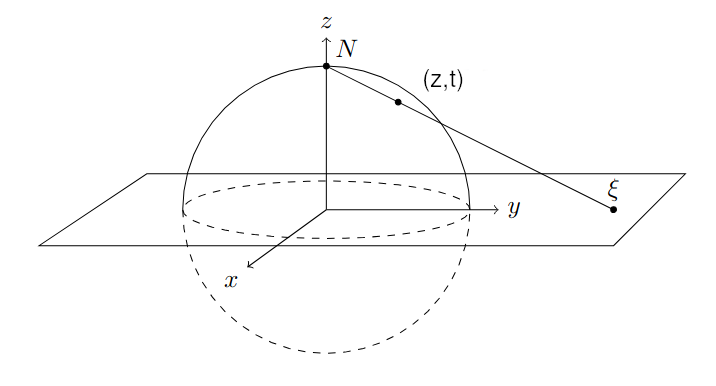
\includegraphics[scale=0.5]{assets/RiemannSphere.png}
    \end{center}
    We can similarly define $\pi_S$ and verify that the images of the
    projections are $X \setminus \set{N}$ and $X \setminus \set{S}$
    accordingly.
    
    Now $X$ is a Riemann surface with an atlas consisting of 
    $\pi_S \colon X \setminus \set{S} \to \C$ and
    $\pi_N \colon X \setminus \set{N} \to \C$.
    We denote the Riemann sphere as $\hat{\C}$.
\end{example}

\begin{definition}[Biholomorphism of Riemann surfaces]
    Let $(X, (U_i, f_i))$, $(Y, (W_i,g_i))$ be two Riemann surfaces.
    A biholomorphism between them is a homeomorphism
    $X \xrightarrow{\phi} Y$ such that $g_i \circ \phi \circ f_i^{-1}$ 
    are biholomorphisms on their domains of definition.
\end{definition}

A main problem in Riemann surfaces was classifying certain types of 
Riemann surfaces up to biholomorphisms.

\begin{theorem}\tt{Riemann mapping theorem}
    Any two proper open simply connected subsets of $\C$ are biholomorphic.
\end{theorem}

A generalization of the Riemann mapping theorem is the uniformization theorem
proved by Kobe in 1907.

\begin{theorem}\tt{Uniformization theorem}
    Any simply connected Riemann surface is biholomorphic to one of the
    following:
    \begin{enumerate}
        \item[(1)] $\C$
        \item[(2)] $\hat{\C}$
        \item[(3)] $\H = \set{z \in \C \colon \mathrm{Im}(z) > 0}$
    \end{enumerate}
\end{theorem}

We will give a proof for this theorem in the end of the class.

A natural question that arises is what about non simply connected Riemann
surfaces?

\begin{theorem}\tt{Uniformization theorem, part II}
    Any connected Riemann surface is biholomorphic either to $\hat{\C}$
    or to a quotient of $\C$ or $\H$ by a properly discontinuous
    torsion-free subgroup of biholomorphisms.
\end{theorem}

\begin{remark}
    Biholomorphisms of $U = \C$ or $\H$ (or any subset of $\C$)
    forms a group under composition.
    We denote that group by $\Bih(U)$.
\end{remark}

\begin{definition}[Properly discontinuous group]
    A countable subgroup of $\Bih(U)$ is said to be properly discontinuous
    if for all compact $K \subseteq U$, the set 
    $\set{g \in G \colon gK \cap K \neq \emptyset}$ is finite.
\end{definition}

\begin{definition}[torsion-free action]
    $G \subseteq \Bih(U)$ is torsion-free if $gp = p$ for some $p \in U$
    implies $g$ is the identity.
\end{definition}

\begin{remark}
  Notice that multiplication in $gp$ is the group action of $g$ on the 
  set $U$. That us $gp = g(p)$.
\end{remark}

We can know define the quotient space $\bigslant{U}{G}$ where
$p \sim q$ if there exists $g \in G$ such that $gp = q$.

Introduce a topology on $\bigslant{U}{G}$ which is the coarsest topology
such that the canonical projections $U \to \bigslant{U}{G}$ are continuous.

Under the assumptions that $G$ is properly discontinuous and torsion-free,
$\bigslant{U}{G}$ is a Riemann surface with the following charts.
By assumptions on $G$, we can find for any $p \in U$ a neighbourhood $W$ of
$p \in U$ such that $\pi \colon U \to \bigslant{U}{G}$ is a homeomorphism
onto its image when restricted to $W$.

So, restrictions of $\pi$ to these neighbourhoods $W$ provide an atlas.

\begin{definition}[Free action]
  Let $G$
\end{definition}

\subsection{Introduction to Teichmuller spaces}
Let $S$ be a topological space.
Then
\[
  \mathrm{Modulispace}(S) = 
  \set{\text{Riemann surfaces homeomorphic to $S$ up to biholomorphisms}}
\]
\begin{definition}[Teichmuller space]
  We consider pairs $(X,f)$ where $X$ is a Riemann space and
  $f \colon S \to X$ is a homeomorphism.
  Then
  \[
    \mathrm{Teich}(S) = 
    \bigslant{\set{(X,f) \colon f \colon S \to X}}{\sim}
  \]
  where $(X_1,f_1) \sim (X_2,f_2)$ if there exists a biholomorphism 
  $X_1 \taking{\phi} X_2$ such that $f_2 \circ f_1^{-1}$ is homotopic to
  $\phi$.
  In other words
  % Triangle
  commutes up to homotopy.
\end{definition}

\begin{remark}
  The pair $(X,f)$ is called a \emph{marking} for $S$.
\end{remark}

\begin{definition}[Homotopy]
  We say that two continuous functions $f$, $g$ from a topological space $X$
  to $Y$ are homotopic if there exists a continuous function 
  $H \colon X \times [0,1] \to Y$ such that $H(x,0) = f(x)$ and
  $H(x,1) = g(x)$ for all $x \in X$.
\end{definition}

\begin{definition}[Mapping class group]
  First we define:
  \begin{align*}
    &\Homeo^+(S) = \set{\text{Orientation preserving homeomorphisms
    $S \to S$}} \\
    &\Homeo^0 \triangleleft \Homeo^+(S) = \set{
      \text{the homeo. homotopic to the identity.}}
  \end{align*}
  And now we define
  \[
    \MCG(S) = \bigslant{\Homeo^+(S)}{\Homeo^0(S)} =
    \frac{\Diff^+(S)}{\Diff^0(S)}.
  \]
\end{definition}

We have that $\MCG$ acts on $\Teich(S)$ by $\varphi \in \Homeo^+(S),
[\varphi] \in \MCG(S)$
as such
\[
  [\varphi] [(X,f)] = [(X,f \circ e^{-1})].
\]

Now $\M(S) = \bigslant{\Teich(S)}{\MCG(S)}$.
Our goal is to determine $\M(S)$ and $\MCG(S)$ when $S$ is a torus.

\begin{theorem}
  Assume $S$ is a torus $T \cong \bigslant{\R^2}{\Z^2}$.
  Then $\MCG(S) = \SL_2(\Z)$ acting linearly on the torus.
  $\M(S)$ can be identified with $\bigslant{\H}{\SL_2(\Z)}$ where the
  action is by Mobius transformations.
\end{theorem}
\begin{proof}
  Any Riemann surfaces homeomorphic to $S$ has to form 
  $\bigslant{\C}{\Lambda}$ where $\Lambda \subseteq \Bih(\C)$ is
properly disc, free, and $\Lambda \ip{z \to z + \tau_1}{z \to z + \tau_2}$
  where $\tau_1,\tau_2 \notin \R$.
  We have to determine when different $\bigslant{\C}{\Lambda}$ are
  biholomorphic.
  We can also write $\bigslant{\C}{\Lambda}$ where 
  $\Lambda = \ip{\tau_1}{\tau_2} \subseteq \C$.
  If $\Lambda_1 = \ip{\tau_1}{\tau_2}$, $\Lambda_2 = \ip{c \tau_1}{c \tau_2}$
  for $c \in \C^*$.
  Then $\bigslant{\C}{\Lambda_1} \to \bigslant{\C}{\Lambda_2}$
  is given by $[z] \to [cz]$.

  For any $\tau_1, \tau_2 \in \C$ there exists $c \in \C^{\times}$
  such that (up to change in order)

  % ADD STUFFFF

  This tells us that any Riemann torus is biholomorphic to 
  $\bigslant{\C}{\ip{XX}{XX}}$ where $\tau \in \H$.

  So we have a surjection $\H \to \M(S)$.
\end{proof}

\begin{theorem}
  $\bigslant{\C}{\ip{1}{\tau_1}}$ is biholomorphic to 
  $\bigslant{\C}{\ip{1}{\tau_2}}$ iff exists $A \in \SL_2(\Z)$
  such that writing $\tau_1, \tau_2$ as elements of $\R^2$, we have
  $A\tau_1 = \tau_2$.
\end{theorem}
\begin{proof}
  Suppose there exists a biholomorphism 
  $f \colon \bigslant{\C}{\ip{1}{\tau_1}} \to \bigslant{\C}{\ip{1}{\tau_2}}$.
  Let $\bar f \colon \C \to \C$ be a lift of $f$.
  This means $f(g + x) - f(x) \in \ip{1}{\tau_1}$ whenever
  $g \in \ip{1}{\tau_1}$.
  \begin{align*}
    &f \colon \bigslant{\C}{\ip{1}{\tau_1}} \to \bigslant{\C}{\ip{1}{\tau_2}}
    bih. \\
    &\bar f \colon \C \to \C lift.
  \end{align*}
  By post composing with a biholomorphism of $\C$ we can assume $\bar f(0) = 0$.
  We know that $\bar f(\tau_2)$ and $\bar f(1)$ are equivalent mod
  $\ip{1}{\tau_1}$.
\end{proof}

%%%% LECTURE 4

\begin{remark}
  Let $S$ be a Riemann surface.
  Recall that $\M(S)$ is the moduli space of $S$, which is the space of Riemann
  surfaces homeo to $S$ up to biholomorphism.
\end{remark}
Recall that we define
\[
  \MCG(S) = \bigslant{\Homeo^+(S)}{\Homeo^0(S)}
\]
And the Teichmuller space of $S$
\[
  \mathrm{Teich}(S) = 
  \bigslant{\set{(X,f) \colon f \colon S \to X}}{\sim}
\]
where $(X_1,f_1) \sim (X_2,f_2)$ if there exists a biholomorphism 
$X_1 \taking{\phi} X_2$ such that $f_2 \circ f_1^{-1}$ is homotopic to $\phi$.

Our goal today is to show that for $T = \text{torus} = \bigslant{\R^2}{\Z^2}$.
\begin{itemize}
  \item $\MCG(S) \cong \SL_2(\Z)$.
  \item $\M(S) \cong \bigslant{\H}{\SL_2(\Z)}$.
  \item $\Teich(S) \cong \H$.
\end{itemize}

Notice that because of the relation
\[
  \bigslant{\Teich(S)}{\MCG(S)} = \M(S)
\]
we only need to prove two of these propositions.

First let's prove that $\M(S) \cong \bigslant{\H}{\SL_2(\Z)}$.
Any Riemann surface is homeomorphic to $T$ (a complex torus) is biholomorphic
to $\bigslant{\C}{\ip{\tau_1}{\tau_2}}$.

Recall that if $c \in \C^{\times}$ then $\bigslant{\C}{\ip{\tau_1}{\tau_2}}$
is biholomorphic to $\bigslant{\C}{\ip{c \tau_1}{c \tau_2}}$ via the map
\[
  f(z + \ip{\tau_1}{\tau_2}) = cz + \ip{c \tau_1}{c \tau_2}.
\]
Up to changing the order of $\tau_1$, $\tau_2$ we can find $c \in \C{\times}$
such that $c \tau_1 = 1$ and $c_2 \in \H$.

Our goal now is to determine when there exists a biholomorphism
\[
  \bigslant{\C}{\ip{1}{\tau_1}} \mapsto
  \bigslant{\C}{\ip{1}{\tau_2}}, \quad \tau_1,\tau_2 \in \H
\]

Denote $\Lambda_{\tau} = \ip{1}{\tau}$, when $\tau \in \H$.

\begin{theorem}
There exists a biholomorphism
\[
  \bigslant{\C}{\ip{1}{\tau_1}} \mapsto
  \bigslant{\C}{\ip{1}{\tau_2}}, \quad \tau_1,\tau_2 \in \H
\]
iff there exists 
\[
  \begin{pmatrix}
    a & b \\
    c & d
  \end{pmatrix} \in \SL_2(\Z)
\]
with $\tau_2= \frac{a \tau_1 + b}{c \tau_2 + d}$.
This will imply that \item $\M(S) \cong \bigslant{\H}{\SL_2(\Z)}$.
\end{theorem}
\begin{proof}
  Suppose there exists a biholomorphism 
  \[
    f \colon \bigslant{\C}{\ip{1}{\tau_1}} \to
    \bigslant{\C}{\ip{1}{\tau_2}}.
  \]
  Lift it up to $\bar f \colon \C \to \C$.
  Then $\bar f(g + x) - \bar f(x) \in \Lambda_{\tau_1}$
  whenever $x \in \C$, $g \in \Lambda_{\tau_2}$.
  We can replace $\bar f$ with $\bar f - \bar f(0)$.
  We can assume that $\bar f(0) = 0$ (and is still a lift off).
  \begin{remark}
    Since $\bar f$ is a lift off of $f$ we have 
    $\bar f(\Lambda_{\tau_2}) = \Lambda_{\tau_1}$.
  \end{remark}
  We know that $\bar f$ has form $\bar f(z) = a z + b$ such that
  $a \in \C^{\times}$, $b \in \C$.
  As $\bar f(0) = 0$ we have $\bar f(z) = a z$.
  Also, $\set{0,1,\tau_2} \subseteq \Lambda_{\tau_2}$ so 
  $0 = \bar f(0), \bar f(1) = a, \bar f(\tau_2) = a \tau_2$ are in
  $\Lambda_{\tau_1}$ so we can write $a = \bar f(1) = $
  %% MOR$E STUFF?
  We now have
  \[
    \tau_2 =
    \begin{pmatrix}
      a & b \\
      c & d
    \end{pmatrix}
  \]
  and we still need to show it is an element of $\SL_2(\Z)$.
  %% THE PART
\end{proof}

\subsection{Isotopy and Homotopy}
Let $X$ be a metric space and $F_0, F_1 \colon X \to X$ homeomorphisms.
Then we say $F_0$, $F_1$ are homotopic if there exists a family $F_t$
for $t \in [0,1]$ of continuous maps such that $t \mapsto F_t(x)$ is
continuous for all $x \in X$ (we don't require $F_0$, $F_1$ to be 
homeomorphisms).

The maps $F_0$, $F_1$ are said to be isotopic if $F_t$ are required to
be homeomorphisms.

For a surface $S$, we defined $\MCG(S)$

\begin{theorem}[Baire, Epstein]
  If $S$ is a finite type surface (e.g.\ closed surface of XXX)
  then two homeomorphisms $F_0, F_1 \colon X \to X$ are homotopic
  iff they are isotopic.
\end{theorem}

Last time we have shown that if $T = \R^2 / \Z^2$ is a torus,
then $\MCG(S) = \SL_2(\Z)$.
For any $A \in \SL_2(\Z)$ we obtained a homeomorphism
\[
  \fullfunction{\psi_A}{T}{T}{[x]}{[Ax]}
\]
We showed that any orientation preserving homeomorphism $\phi \colon T \to T$
is homotopic to $\psi_A$ for some $A \in \SL_2(\Z)$.

This gives a map
\[
  \fullfunction{\Phi}{\SL_2(\Z)}{\MCG(T)}{[A]}{[\psi_A]}
\]
which we know is surjective.
Why is $\Phi$ injective?


We want to show that for $A \in \SL_2(\Z)$ and $A \neq I$ that $\psi_A$
is not homotopic to the identity map.

We will see this by showing that $\psi_A$ acts nontrivially on the fundamental
group $\Pi_1(T)$.

\begin{definition}[Loop]
  A loop based at $p$ is a continuous function $\gamma \colon [0,1] \to X$ with 
  $f(0) = f(1) = 0$.
\end{definition}

\begin{definition}[Homotopy]
  We say that two continuous functions $f$, $g$ from a topological space $X$
  to $Y$ are homotopic if there exists a continuous function 
  $H \colon X \times [0,1] \to Y$ such that $H(x,0) = f(x)$ and
  $H(x,1) = g(x)$ for all $x \in X$.
\end{definition}

\begin{definition}[Fundamental group]
  The fundamental group of a topological space $X$ is the space of all loops
  in $X$ based at a point $p \in X$ up to homotopy.
\end{definition}
 
A homeomorphism $\psi \colon X \to X$ acts on $\Pi_1(X)$ by
\[
  \psi[\gamma] = [\psi \circ \gamma].
\]
The group operation is concatenation of loops.

Invesrion is changing the direction of the loop.

\begin{exercise}[Fundamental group of the torus]
  The fundamental group of $T$ is $\Pi_1(T) \cong \Z^2$ is generated
  by \[\left[\begin{pmatrix} 1 \\ 0 \end{pmatrix}\right] \tand
  \left[\begin{pmatrix} 0 \\ 1 \end{pmatrix}\right].\]
  This means any loop is homotopic to
  $[\begin{pmatrix} a \\ b \end{pmatrix}]$
  by doing $[\begin{pmatrix} 1 \\ 0 \end{pmatrix}]$ $a$ times
  and $[\begin{pmatrix} 0 \\ 1 \end{pmatrix}]$ $b$ times.
\end{exercise}

For $A \in \SL_2(\Z)$ and $\psi_A \colon T \to T$ action on
$\Pi_1(T, (0,0))$ (fundamental group of the torus based in $(0,0)$)
defined by
\[
  (x,y) \mapsto A \begin{pmatrix} x \\ y \end{pmatrix}.
\]
If $\psi_A$ was homotopic to the identity it owuld act trivially on
$\Pi_1(T, (0,0))$ which means that
\[
  [0,1] = [A (1,0)] = [(b,d)] \stand [(1,0)] = [A(1,0)] = [(a,c)]
\]
so $(a,c) = (1,0)$ and $(b,d) = (0,1)$ so $A$ is the identity matrix.

\subsection{Hyperbolic geometry}
Recall that $\Bih(\H)$ is the set of Mobius transformations with a representing
matrix in $\SL_2(\Z)$.

But $z \mapsto \frac 1z$ does not present Euclidean metric on 
$\H = \set{z \colon \Im(z) > 0}$.

We will introduce a metric $\rho = \rho_{hyp}$ on $\H$ s.t.\
\[
  \Bih(\H) = \text{Orientation preserving isometrics of } (\H,\rho).
\]

\begin{definition}[Length]
  Let $\gamma \colon [0,1] \to \H$ be a pointwise continuous smooth path
  between $a$ and $b$.

  The hyperbolic length of $\gamma$ is
  \[
    L_{\rho}(\gamma) :=
    \int_0^1 
  \]
\end{definition}

%%%%%%%%

Recall that every element in every $\Mob(\hat \C)$ is conjugate
to either $z \mapsto z + 1$ or $z \mapsto \Lambda z$ for
$\Lambda \in \C \setminus \set{0,1}$.

Recall that $T_{\lambda}(z)= \Lambda z$ and
$T_{\Lambda^{-1}}(z) = \Lambda^{-1} z$ are conjugate via the transform
\[
  S(z) = \frac{1}{z}.
\]
Indeed this can be verified.

So in the above classification we can assume $|\Lambda| \geq 1$.

\begin{corollary}
  A complete set of nonindentity conjugacy class representations in $\Mob(\C)$
  is $z \mapsto z + 1$ or $z \mapsto \Lambda z$ for $\set{\Lambda, 1 / \Lambda}$
  distinct unordered pairs.
\end{corollary}
\begin{proof}
  We know that $z \mapsto z + 1$ cannot be conjugate to $z \mapsto \Lambda z$
  which has two fixed points in $\hat \C$.

  We need to show that for different $\Lambda \neq 1$ and $|\Lambda| \geq 1$,
  $z \mapsto \Lambda z$ are not conjugate.

  Recall that in general if $\psi \in \Mob(\hat \C)$ then
  \[
    \psi = \psi_A(z) = \frac{a z + b}{c z + d} \st
    A =
    \begin{pmatrix}
      a & b \\
      c & d
    \end{pmatrix} \in \SL_2(\C).
  \]
  There are two matrices representing $\psi$ which are $A$ and $-A$.

  Since $\PSL_2(\C) \to \Mob(\hat \C)$ defined as $[A] \mapsto \psi_A$
  is an isomorphism, we know that $\psi_A$ and $\psi_B$ are conjugate
  in $\Mob(\hat C)$ if and only if $A$ is conjugate to $\pm B$ in
  $\SL_2(\C)$.

  Now, if $A$ is conjugate to $B$ then $A$, $B$ have the same eigenvalues.

  Coming back to $z \mapsto \Lambda z$.

  If $\Lambda_1, \Lambda_2 \in \C \setminus{0,1}$ such that
  $|\Lambda_1|, |\Lambda_2| \geq 1$. $z \mapsto \Lambda z$ is represented
  by
  \[
    \begin{pmatrix}
      \Lambda & 0 \\
      0 & 1 / \Lambda
    \end{pmatrix} \in \SL_2(\C).
  \]
  which has eigenvalues $(1, 1 / \Lambda)$ for distinct $|\Lambda| \geq 1$
  so they can't be conjugate.
\end{proof}

\subsection{Qualitative properties of M\"obius transformations}

The map $z \mapsto z + 1$ preserves the unique line in $\H$ which converges
to $\infty$ (which is the fixed point of $z \mapsto z + 1$) in both directions. 
In other words, all the horizontal lines.

The map $z \mapsto \Lambda z$ preserves the geodesic in $\H$ which converges to
the two fixed points $z \to \Lambda z$ (namely $0$, $\infty$).

% More things I don't know
\begin{proposition}
  Any discrete subgroup of $\R$ is c$\Z$ for $c \in \R$.
  In this case it is infinite cyclic.
\end{proposition}
\begin{proposition}
  Any discrete subgroup of the circle $S^1$ is 
  $\set{e^{\frac{2 \pi i k}{n}} \colon k = 0,1,\dots,n-1}$
  In this case it is finite cyclic.
\end{proposition}


Recall that for $g \in \PSL_2\R$ the commutator of $g$ is
$C_{\PSL_2\R}(g) = \set{h \in \PSL_2\R \colon hg = gh}$.

\begin{theorem}
  If $g \in \PSL_2\R$ is a (hyperbolic / parabolic / elliptical)
  then $C_{\PSL_2\R}(g)$
  consists of the idnetity with all the
  (hyperbolic / parabolic / elliptical) elements which have the
  same fixed point set in
  $\bar \H = \H \cup \R \cup \set{\infty}$.
\end{theorem}

\begin{remark}
  The requirement (hyperbolic / parabolic / elliptical) is
  redundant.
\end{remark}

Recall that if $g$ is parabolic then $C_{\PSL_2\R}(g)$ is
conjugate to
\[
  C_{\PSL_2\R}(z \mapsto z + 1) =
  \set{z \mapsto z + r \colon r \in \R}.
\]

If $g$ is elliptic then $C_{\PSL_2\R}(g)$ is
conjugate to
\[
  C_{\PSL_2\R}\del{z \mapsto 
  \frac{(\cos \theta) z - \sin \theta}
  {(\sin \theta) z + \cos \theta}} =
  \set{z \mapsto \frac{(\cos \theta) z - \sin \theta}
  {(\sin \theta) z + \cos \theta} \colon \theta \in [0,2 \pi)}.
\]
If $g$ is hyperbolic \dots

\begin{theorem}
  If $\Gamma \subseteq \PSL_2\R$ is discrete, and each nonidentity
  element of $\Gamma$ has the same fixed point set then
  $\Gamma$ is cyclic.
\end{theorem}
\begin{proof}
  If all nonidentity elements of $\Gamma$ have the same fixed
  point set then they are either all hyperbolic, all parabolicm
  or all elliptic.
  \begin{enumerate}
    \item[(1)] In case they are all hyperbolic,
      \[
        \mathrm{fix}(\Gamma) = \set{p,q} \subseteq \partial \H
      \]
      Then after conjugating by $T \in \Mob(\H)$ with \dots
  \end{enumerate}
\end{proof}

\newpage
\section{Function Theory 2}
\subsection{Introduction}
\begin{definition}[The $H^{\infty}(U)$ class]
  Let $U$ be an open subset of $\C$.
  We denote the class of analytic functions on $U$
  by $H(U)$ and define the following class of functions
  \[
    H^{\infty}(U) :=
    \set{f \in H(U) \colon \norm{f}_{\infty} = \sup_{z \in U}
    \abs{f(z)} < \infty}.
  \]
\end{definition}

\begin{definition}[Schur class]
  We define the following class of functions
  \[
    S := \set{f \in H^{\infty}(\D) \mid \norm{f}_{\infty} \le 1}.
  \]
\end{definition}

\begin{proposition}[Schwartz's--Pick lemma]
  \label{prop:schwartz-pick}
  Let $f \in S$ and let $z_1,z_2 \in S$.
  Then
  \[
    \abs{\frac{f(z_1) - f(z_2)}{1 - f(z_1) \overline{f(z_2)}}} \le
    \abs{\frac{z_1 - z_2}{1 - z_1 \overline{z_2}}}.
  \]
\end{proposition}
\begin{proof}
  To be added.
\end{proof}
\begin{remark}
  \Cref{prop:schwartz-pick} is also known as the invariant form of
  the Schwartz lemma.
\end{remark}

\begin{definition}[Pseudohyperbolic metric]
  Let $z,w \in \D$.
  We define the pseudohyperbolic metric by
  \[
    \rho(z,w) := \abs{\frac{z - w}{1 - \overline{w} z}}.
  \]
\end{definition}
\begin{remark}
  The map $\rho$ is invariant under M\"obius transformations.
  That is, if $\phi$ is a M\"obius transformation so that $\phi(w) = 0$
  then we have $\rho(z,w) = \abs{\phi(z)}$.
\end{remark}

\begin{remark}
  Let $f \colon \D \to \D$.
  Then from the Schwartz's--Pick lemma we have
  \[
    \rho(f(z),f(w)) \le \rho(z,w).
  \]
  This means that $f$ is a contraction.
  Moreover, there is an equality if and only if $f$ is
  an automorphism of the disc.
  That is because if $f$ is an automorphism of the disc then $f$ and
  $f^{-1}$ are both contractions which implies the equality.
\end{remark}

\begin{problem}[Pick's interpolation problem]
  \label{problem:picks-interpolaltion-problem}
  Let $z_1,\dots,z_n \in \D$ and let
  $w_1,\dots,w_n \in \D$.
  Does there exist a function 
  $f \in H(\D)$ so that
  $f(z_i) = w_i$ for all $1 \le i \le n$
  and $\abs{f(\lambda)} \le 1$ for all $\lambda \in \D$?
\end{problem}
\begin{remark}
  In case $n = 1$ we can solve the function immediately by
  using $f = \psi_{w_1} \circ \psi_{z_1}$ which first interchanges between
  $0$ and $z_1$ then by $0$ and $w_1$ so $f(z_1) = w_1$ as wanted.
  
  In case $n = 2$ we can do this if and only if
  $\rho(w_1,w_2) \le \rho(z_1,z_2)$.
  An equivalent statement is that
  \[
    \begin{bmatrix}
      \frac {1-|z_{1}|^{2}}{1-|w_{1}|^{2}} &
      \frac {1-{\overline {z_{1}}}z_{2}}{1-{\overline {w_{1}}}w_{2}}
    \\[5pt]
      \frac {1-{\overline {z_{2}}}z_{1}}{1-{\overline {w_{2}}}w_{1}} &
      \frac {1-|z_{2}|^{2}}{1-|w_{2}|^{2}}
    \end{bmatrix}
    \geq 0.
  \]
  % that is because?
\end{remark}

\begin{theorem}[Pick's theorem]
  \label{thm:pick}
  Let $z_1,\dots,z_n \in \D$ and let
  $w_1,\dots,w_n \in \D$.
  Then there exists $f \in H(\D)$ so that
  $f(z_i) = w_i$ for all $1 \le i \le n$ if and only if
  the \textit{Pick matrix}:
  \[
    \begin{bmatrix}
      \cfrac{1 - w_i \overline{w_j}}{1 - z_i \overline{z_j}}
    \end{bmatrix}_{i,j=1}^{n}
  \]
  is positive-semidefinite.
\end{theorem}
\begin{proof}
  When $n = 1$ the condition is that
  \[
    \cfrac{1 - w \overline{w}}{1 - z \overline{z}} \geq 0
  \]
  which holds for any $z,w \in D$.
  When $n = 2$ the condition is that
  \[
    \begin{bmatrix}
      \cfrac{1 - \abs{w_1}^2}{1 - \abs{z_1}^2} &
      \cfrac{1 - w_1 \overline{w_2}}{1 - z_1 \overline{z_2}}
      \\
      \cfrac{1 - w_2 \overline{w_1}}{1 - z_2 \overline{z_1}} &
      \cfrac{1 - \abs{w_2}^2}{1 - \abs{z_2}^2}
    \end{bmatrix} \geq 0
  \]
  which reduces to
  $\rho(w_1,w_2) \le \rho(z_1,z_2)$.
\end{proof}

\begin{definition}[Hardy space]
  We define the Hardy space $H^2(\D)$ as followsing
  \[
    H^2(\D) = H^2 =
    \set{h(z) = \sum_{n=0}^{\infty} a_n z^n \in H(\D) \st
    \norm{h}_2^2 := \sum \abs{a_n}^2 < \infty}.
  \]
\end{definition}
\begin{remark}
  Given a power series $\sum a_n z^n \in H^2$ we have by
  the Cauchy--Scwarz's inequality
  \[
    \abs{\sum a_n z^n} \le
    \del{\sum \abs{a_n}^2}^{1/2}
    \del{\sum \abs{z}^{2n}}^{1/2}
  \]
  which converges for any $z \in \D$.
\end{remark}

\begin{definition}[Inner product]
  Given two formal sums we define their inner product to be
  \[
    \ip{a}{b} =
    \ip{\sum a_n z^n}{\sum b_n z^n}_{H^2} =
    \norm{\sum a_n \overline{b^n}} \le
    \norm{a}_2 \norm{b}_2
  \]
\end{definition}
% define norm and metric

\begin{remark}
  The space $H^2$ is a complete metric space and an inner
  product space so it is a Hilbert space.
\end{remark}

\begin{definition}[Szego kernel]
  The Szego kernel is a function
  $K \colon \D \times \D \to \C$
  defined by
  \[
    K(z,w) := \frac{1}{1 - z \overline{w}}
  \]
  and the kernel function at $w \in \D$ is
  \[
    k_w(z) = k(z,w) = \frac{1}{1 - z \overline{w}}.
  \]
\end{definition}

\begin{proposition}
  Let $k_w \in H^2$,
  let $w \in \D$
  and let $h \in H^2$.
  Then $h(w) = \ip{h}{k_w}$
  and consequently from the Cauchy--Schwarz inequality we obtain
  $\abs{h(w)} \le \frac{1}{\sqrt{1 - \abs{w}^2}} \norm{h}_2$.
\end{proposition}
\begin{proof}
  We have that
  \[
    k_w(z) = k(z,w) = \frac{1}{1 - z \overline{w}}.
  \]
  to be added
\end{proof}

\begin{definition}[Bounded operator]
  Let $X$, $Y$ be normed spaces
  and let $T \colon X \to Y$ be a linear function.
  Then $T$ is said to be bounded if and only if $\norm{T} < \infty$.
  We denote $B(X,Y)$ the space of bounded operators from $X$ to $Y$.
\end{definition}
\begin{remark}
  The dual space of $X^*$ is $X^* = B(X,\C)$.
\end{remark}

\begin{remark}
  Let $w \in \D$ and define
  $ev_w \colon H^2 \to \C$ by
  $ev_w(h) = h(w) = \ip{h}{k_w}$ or $h \mapsto h(w)$.
  The evaluation map of the Hardy space $ev_w \colon H^2 \to \C$ is bounded.
\end{remark}

\begin{definition}[Reproducing kernel Hilbert space]
  Let $H$ be a linear subspace of the space of functions from $X$ to $\C$.
  Then $H$ is said to be a RKHS if $H$ is a Hilbert space and
  point evaluation $ev_x$ is bounded for all $x \in X$.
\end{definition}

By Riesz theorem for all $\phi \in H^*$ there exists $g \in G$
so that for all $h \in H$ we have $\phi(h) = \ip{h}{g}$.
Then %???

\begin{definition}[Kernel function]
  
\end{definition}

% the kernel is semi positive definite

\begin{definition}[Multiplier algebra]
  Let $H$ be an RKHS on $X$.
  Then the multiplier algerba on $H$ is the space
  \[
    \Mult(H) :=
    \set{f \colon X \to \C \mid h \in H \implies f h \in H}.
  \]
\end{definition}

% M_f

\begin{question}
  Can we compute $\Mult(H^2)$?
\end{question}
\begin{answer}
  We know that all polynomials are in $\Mult(H^2)$.
\end{answer}

\begin{proposition}
  \label{prop:temp}
  Let $H$ be a RKHS on $X$ and let $f \in \Mult(H)$.
  Then for all $x \in X$ we have $M_f^* k_x = \overline{f(x)} k_x$.
  Conversely, if $T \in B(H)$ then
  $T k_x = \lambda_x K_x$ which implies that $T = M_f^*$
  and $f \in \Mult(H)$.
\end{proposition}

\begin{corollary}
  Every multiplier is a bounded function
  \[
    \abs{f(x)} \le \norm{M_f^*} = \norm{M_f}.
  \]
\end{corollary}
\begin{corollary}
  We have that $\Mult(H^2) \subseteq H^{\infty}(\D)$
  since $\norm{f}_{\infty} \le \norm{f}_{\Mult}$.
\end{corollary}

\begin{proofof}{\Cref{prop:temp}}
  Let $h \in H$ and let $f \in \Mult(H)$.
  Then
  \begin{align*}
    f(x) h(x) &= \ip{fh}{k_x} \\
              &= \ip{M_f h}{k_x} \\
              &= \ip{h}{M_f^* k_x}.
  \end{align*}
\end{proofof}

% needs rewriting

\begin{definition}[Multiplication algebra norm]
  We define for $f \in \Mult(H)$
  \[
    \norm{f}_{\Mult} :=
    \norm{M_f} =
    \sup_{h \neq 0} \frac{\norm{M_f h}}{\norm{h}} < \infty
  \]
\end{definition}

\begin{proposition}
  Let $H$ be a RKHS on $X$ and $t \in B(H)$
  Then we have 
  \[
    \forall x \in X \quad \exists \lambda_x \in \C \st T K_x = \lambda_x K_x
    \iff
    \exists f \in M(H) \st T = M^*_{f}
  \]
  and in this case $\lambda_x = \overline{f(x)}$.
\end{proposition}

\begin{definition}
  Let $f \colon \D \to \C$ and let $r \in (0,1)$.
  Then we define $f_r(z) = f(rz)$.
\end{definition}
\begin{remark}
  If $f \in H^2$ then $f_r \in H^2$.
  This is because if $f(z) = \sum_{n=0}^{\infty} a_n z_n$
  then we have $f_r(z) = \sum_{n=0}^{\infty} r^n b_n z_n$. %b_n or a_n.
\end{remark}

\begin{proposition}
  Let $f(z) = \sum_{n=0}^{\infty} a_n z_n$.
  Then
  \[
    \norm{f}_{2}^{2} =
    \sum \abs{a_n}^2 =
    \lim_{r \nearrow 1}
    \frac{1}{2\pi} \int_{0}^{2\pi} \abs{f_r\del{e^{it}}}^2 \dt.
  \]
\end{proposition}
\begin{remark}
  We also have that
  \[
    \norm{f}_{2}^{2} =
    \int_{T} \abs{f}^2 \dm
  \]
  where $m$ is the Lebesgue measure on the circle.
\end{remark}
\begin{proof}
  to be added.  
\end{proof}

\begin{proposition}
  Let $f \in H^{\infty}$ and $h \in H^2$.
  We have
  \[
    \norm{f h}_{2}^{2} =
    \lim_{r \nearrow 1}
    \frac{1}{2\pi}
    \int_{0}^{2\pi} \abs{f_r\del{e^{it}} h_r\del{e^{it}}}^2 \dt \le
    \norm{f}^2_{\infty} \norm{h}_{2}^{2}
  \]
  which implies that $f \in \Mult(H)$.
  We also have $\norm{f}_{\Mult} = \norm{M_f} \le \norm{f}_{\infty}$.
\end{proposition}
\begin{corollary}
  We get that $\Mult(H^2) = H^{\infty}$.
\end{corollary}

\begin{theorem}[Pick's theorem]
  \label{thm:pick-again}
  Let $z_1,\dots,z_n \in \D$ and let
  $w_1,\dots,w_n \in \D$.
  Then there exists $f \in H(\D)$ so that
  $f(z_i) = w_i$ for all $1 \le i \le n$ if and only if
  the \textit{Pick matrix}:
  \[
    \begin{bmatrix}
      \cfrac{1 - w_i \overline{w_j}}{1 - z_i \overline{z_j}}
    \end{bmatrix}_{i,j=1}^{n}
  \]
  is positive-semidefinite.
\end{theorem}
\begin{proof}
  Let $z_1,\dots,z_n \in X$ and $w_1,\dots,w_n \in \C$.
  Let $H$ be an RKHS on $X$ so that $H = H^2$.
  If there exists $f \in \Mult(H)$ so that
  \begin{enumerate}
    \item[(1)] $\norm{f}_{\Mult} \le 1$;
    \item[(2)] $f(z_i) = w_i$
  \end{enumerate}
  then
  \[
    \begin{bmatrix}
      K(z_i,z_j) (1 - w_i \overline{w_j})
    \end{bmatrix} \geq 0.
  \]
  That is because
  \[
    \norm{M_f^*} = \norm{M_f} = \norm{f}_{\Mult} \le 1
  \]
  ...to be added
  The opposite direction holds if we assume that the kernel is of
  the form $K(z,w) = \frac{1}{1 - z \overline w}$.
\end{proof}

\begin{theorem}
  We have that $f \in \Mult(H)$ so that $\norm{f}_{\Mult} \le 1$
\end{theorem}

\begin{definition}[Harmonic function]
  Let $u \in C^2(\Omega)$ where $\Omega$ is a region in $\C = \R^2$.
  Then $u$ is said to be harmonic if $\Delta u = u_{xx} + u_{yy}$.
\end{definition}

\begin{proposition}
  A real $u$ on a simply connected region $\Omega$ is harmonic if and only
  if there exists $f \in f \in H(\Omega)$ so that $u = \Re(f) = \Im(i f)$
\end{proposition}
\begin{proof}
  Let $f = u + iv \in H(\Omega)$.
  From the Cauchy--Riemman equations we get $u_x = v_y$ and $v_x = -u_y$
  which means that $u_{xx} + u_{yy} = v_{yx} - v_{xy} = 0$.

  Next suppose that $u$ is harmonic.
  Define
  \[
    V(x,y) :=
    \int v_x \dx + v_y \dy =
    \int_{\Gamma} -u_y \dx + u_x \dy.
  \]
  Using Green's theorem we get that
  \[
    \int_{\partial \Omega} -u_y \dx + u_x \dy =
    \int_{\Omega} \underbrace{\del{u_{xx} + u_{yy}}}_{=\,0} \dx \dy = 0
  \]
  After integrating $V$ we get that
  \begin{gather*}
    \diffp{V}{x}(x,y) =
    \lim_{h \to 0} \frac{1}{h} \int_{x}^{x+h} -u_{y}(t,y) \dt =
    -u_{y}\vert_{(x,y)}
  \end{gather*}
  which completes the proof.
\end{proof}

\begin{corollary}
  Harmonic functions are $C^{\infty}$.
\end{corollary}
\begin{proof}
  % Suppose $U$ is harmonic in $(1+\epsilon) \D$.
  % We have that
  % \[
  %   u = \Re f \tand
  %   f(z) = \sum_{n=0}^{\infty} a_n z^n.
  % \]
  % We can now write
  % \[
  %   u = \frac{f + \overline f}{2} =
  % \]
\end{proof}

\begin{theorem}
  Let $f \in \L^1(T)$ and let $Hf$ be defined on the closed unit disc
  $\overline \D$ by
  \[
    (Hf)(r e^{i \theta}) =
    \begin{cases}
      f(e^{i \theta}), &r = 1 \\
      P[f](r e^{i \theta}), &0 \le r < 1
    \end{cases}.
  \]
  Then $Hf$ is harmonic in $\D$ and $Hf \in C(\overline D)$
\end{theorem}
\begin{remark}
  This solves the Dirichlet's problem.
\end{remark}
\begin{proof}

\end{proof}






\end{document}
